\documentclass[11pt,a4paper,ngerman]{article}
\usepackage[T1]{fontenc} 
\usepackage[latin1]{inputenc} 
\usepackage{babel}
\usepackage{ae}
\usepackage{bchart}
\usepackage{pgfplots}
\usepackage{float}
\usepackage{ulem}
\usepackage{tikz}
\usetikzlibrary{arrows,shapes,positioning,shadows,trees}
%tikz-setup for drawing trees
\tikzset{
  basic/.style  = {draw, text width=2cm, drop shadow, font=\sffamily, rectangle},
  root/.style   = {basic, rounded corners=6pt, thin,align=center, fill=green!60,
                   text width=8em},
  level 2/.style = {basic, rounded corners=6pt, thin,align=center, fill=green!60,
                   text width=8em},
  level 3/.style = {basic, thin, align=left, fill=pink!60, text width=6.5em}
}
%
%
\usepackage{fancyref}
\usepackage{fancyhdr} 
\usepackage{xcolor}
\usepackage{framed}
\usepackage{url}
\usepackage{makeidx}
\makeindex
\usepackage{listings}
%
%Colors
\definecolor{shadecolor}{rgb}{0.9,0.9,0.9}
% PDF settings
\usepackage[pdfstartview=FitH,pdftitle={Messung der Informationstypen-H�ufigkeiten in der Python-Dokumentation },pdfauthor={Sven Wildermann}, colorlinks=true, linktocpage]{hyperref}
% colorlinks=false, pdfborder={0 0 0} = keine farbigen Links
%
% Header and Footer Style
\pagestyle{fancy}
\fancyhead{}
\fancyhead[R]{\slshape Sven Wildermann}
\fancyhead[L]{\slshape\nouppercase{\rightmark}}
\fancyfoot{}
\fancyfoot[C]{\thepage}
\renewcommand{\headrulewidth}{0pt}
\renewcommand{\sectionmark}[1]{\markright{\thesection\ #1}} 
%
% No identation
\setlength\headheight{15pt}
\setlength\parindent{0pt} 
%
% Custom commands
\newcommand\zb{z.\,B.\ }
\renewcommand\dh{d.\,h.\ }
\newcommand\parbig{\par\bigskip}
\newcommand\parmed{\par\medskip}
\newcommand{\mailto}[1]{\href{mailto:#1}{#1}}
%
% Python Code Listing Style
\definecolor{darkblue}{rgb}{0,0,.6}
\definecolor{darkgreen}{rgb}{0,0.5,0}
\definecolor{darkred}{rgb}{0.5,0,0}
\lstset{language=Python, basicstyle=\ttfamily\small\upshape, commentstyle=\color{darkgreen}\sffamily, keywordstyle=\color{darkblue}\rmfamily\bfseries, breaklines=true,tabsize=2,xleftmargin=3mm, xrightmargin=3mm,numbers=none,frame=single,stringstyle=\color{darkred},
showstringspaces=false}
%
% Titel and author 
\title{
\includegraphics[width=0.6\textwidth]{pictures/logo}\\
{\normalsize Bachelorarbeit am Institut f�r Informatik der Freien Universit�t Berlin, Arbeitsgruppe Software Engineering}\\[6ex]
Messung der Informationstypen-H�ufigkeiten in \newline der Python-Dokumentation}

\author{Sven Wildermann\\
{\normalsize Matrikelnummer: 4567553}\\
{\normalsize \mailto{bachelorarbeit@wildermann.berlin}}\\\\
{\normalsize Betreuer und Gutachter:  Prof. Dr. Lutz Prechelt}\\
{\normalsize Zweitgutachterin: Prof. Dr. Fehr }}

\date{Berlin, 12. August 2014}


\begin{document}

\begin{titlepage}

\pagenumbering{alph}
\maketitle
\thispagestyle{empty}

\vfill{}



\vfill{}

\end{titlepage}

\pagestyle{empty}
\clearpage\pagenumbering{roman}

\section*{Zusammenfassung}
Walid Maalej und Martin P. Robillard haben im September 2013 einen Artikel \cite{MaalejRobillard} ver�ffentlicht, in dem sie die Dokumentationen der Programmiersprachen Java und .NET auf ihren Informationsgehalt hin untersucht und verglichen haben. Diese Untersuchung wird im Rahmen dieser Bachelorarbeit auf die Dokumentation von \href{https://www.python.org/}{Python}\footnote{https://www.python.org/} mit einigen Abweichungen �bertragen. \\
Die von Maalej und Robillard eingef�hrte Taxonomie der in Dokumentationen anzutreffenden Wissenstypen wurde hierf�r auf die Eigenheiten von Python angepasst. Die Einordnung von Teilen der Dokumentationen zu den verschiedenen Wissenstypen wird von Gutachtern im Rahmen eines Forschungspraktikums geleistet und erfolgt mit Hilfe eines eigens hierf�r geschriebenen Werkzeuges. \\
Die anschlie�ende Auswertung der Ergebnisse und Vergleich dieser mit denen aus dem Originalartikel zeigt, dass die vorgenommenen �nderungen in der Konzeption sinnvoll waren und f�r noch eindeutigere Ergebnisse gesorgt haben. Die Struktur der Wissenstypen in der Dokumentation von Python �hnelt stark der bei Java und .NET gefundenen, hat aber auch �berraschende Abweichungen. Die erhobenen Grundlagen bieten zudem eine Grundlage f�r weiteregehende Untersuchungen zu den Informationstypen in der Python-Dokumentation wie beispielsweise die Reihenfolge oder die Wortmenge von Informationen. 


%
%Dieses wurde mit Hilfe des auf Python basierenden Webframeworks \href{https://www.djangoproject.com/}{Django} umgesetzt. 
%
%
%
%F�r die Aufteilung der HTML-Gesamtdokumentation in kleinere Teile und den Import in die Datenbank wurde ein Python-Skript angefertigt, welches f�r die Syntaxanalyse das Paket \href{http://www.crummy.com/software/BeautifulSoup/}{BeautifulSoup4} verwendet. Die statistische Auswertung erfolgte ebenfalls mit Python. Die Ergebnisse werden wo m�glich in Bezug auf die vorhergehende Studie vergleichen und interpretiert.
\section*{Danksagungen}

Zuerst m�chte ich Prof. Dr. Lutz Prechelt f�r die intensive Betreuung und Begutachtung dieser Arbeit danken.
Weiterhin m�chte ich den Studenten der Freien Universit�t Berlin Jakob Warkotsch, Josephine Mertens, Jakob Lennart D�hrsen, Leon Martin George, Malte Detlefsen, Michael Christian Koeck und Robert Kappler f�r die Datenerhebung ebenso danken wie Holger Schmeisky und Franz Zieris von der AG Software Engineering. Dank auch an Christian Salzmann vom technischen Support des Instituts f�r Informatik an der Freien Universit�t Berlin. Mein besonderer Dank geht an Phil Stelzer f�r die Unterst�tzung in der Webentwicklung. Au�erdem m�chte ich meiner Ehefrau Anne Stephanie Wildermann f�r die geistige Unterst�tzung w�hrend der Erstellung dieser Arbeit und f�r die Studienjahre danken. Meinen Eltern und Schwiegereltern danke ich f�r die Unterst�tzung w�hrend meiner gesamten Studienzeit.



\subsection*{Eidesstattliche Erkl�rung}

Ich versichere hiermit an Eides statt, dass diese Arbeit von niemand anderem als meiner Person verfasst worden ist. Alle verwendeten Hilfsmittel wie Berichte, B�cher, Internetseiten oder �hnliches sind im Literaturverzeichnis angegeben, Zitate aus fremden Arbeiten sind als solche kenntlich gemacht. Die Arbeit wurde bisher in gleicher oder �hnlicher Form keiner anderen Pr�fungskommission vorgelegt und auch nicht ver�ffentlicht.
\parbig
12. August 2014 \\ \\ \\
Sven Wildermann 
\setcounter{tocdepth}{5}
\setcounter{secnumdepth}{5}

\tableofcontents
\listoffigures
\clearpage\pagenumbering{arabic}
\pagestyle{fancy}
\setcounter{page}{0}

\section*{Offtopic: Verbesserungen f�r die Bachelorarbeit}

\begin{enumerate}
\item \sout{Ein DOM-Knotenbaum einer typischen HTML-Datei einbauen}
\item \sout{UML-Diagramm des Tools} ergibt wenig Sinn wegen Django
\item \sout{Datenbank-Eintit�ten aufzeigen} Nur wenn noch Zeit �brig ist
\item \sout{M�glicher Workflow (als Nicht-deterministischer Automat oder so)} daf�r nicht komplex genug
\item \sout{Screenshot z.B. von Dokumentationseinheit1898 hinzuf�gen, um das Interface zu zeigen}
\item \sout{Alle Links als Fussnoten anzeigen - sieht besser aus und ist besser f�r den offline-Gebrauch!} 
\item \sout{Nummerierung bei den Code-Schnipseln hinzuf�gen}
\item \sout{Bei Bildern immer Bildunterschriften einf�gen, die etwas zu dem gezeigten aussagen}
\item Alle Kommentare im Code (und den code selbst) auf Rechtschreibfehler �berpr�fen
\item Related Work 
\item Future Work
\item \sout{Wort "Klassifizierung" statt " Typisierung"} Es bleibt bei Typisierung
\item \sout{Links im Literaturverzeichnis anzeigen lassen}
\item HTML-Fehler in der Original-Dokumentation aufzeigen (mindestens 2)
\item HASH-Wert des Quellcodes abdrucken
\item \sout{Alle geschriebenen Kommandos erw�hnen?} Neee zu viel
\item \sout{Stichprobe von Robert erw�hnen} 
\item Passiv vermeiden! 
\item Zusammenfassung: Auf Resultate eingehen (daf�r aber nicht auf bs4 etc.)
\item Mit der Goldstrichprobe vergewissern: Wie oft waren die Studenten sich f�lschlicherweise einig? Damit findet man einen stochastischen Fehler.
\item Umstimmigkeiten nach Kategorien?! 
\item Bild von dem Cado-Tool rein stellen (damit der Vergleich mit dem jetztigen Tool besser gelingt)
\item Kookurrenz noch einmal �berdenken: Ist das so richtig berechnet? Durch den falschen Wert geteilt! (oder?)







\end{enumerate}
\section{Einleitung}
Zu jeder Programmiersprache geh�rt eine Dokumentation �ber die bereitgestellten Funktionalit�ten, auch Referenzhandbuch genannt. 
W�hrend die Vor- und Nachteile der Programmiersprachen h�ufig disktutiert werden, findet man nur wenig Analyse zu den Dokumentationen.
Dabei tr�gt eine Dokumentation nicht unwesentlich zum Erfolg oder Misserfolg einer Programmiersprache bei. Entscheidend ist, wie gut 
die Entwickler mit den gebotenen Informationen zurechtkommen und wie schnell Antworten auf Benutzungsfragen gefunden werden k�nnen. 
Die Anzahl und Qualit�t der Programmbeispiele ist dabei mindestens genauso wichtig wie die Erl�uterung von Funktionalit�ten, Konzepten und Abh�ngigkeiten. 
\newline
Um etwas �ber die Qualit�t von Dokumentationen aussagen zu k�nnen, muss erst einmal verstanden werden, welche Informationen zu welchen Teilen in dem jeweiligen Handbuch vorhanden sind. Der erste Teil dieser Frage wurde bereits von den Walid Maalej und Martin Robillard \cite{MaalejRobillard} beantwortet. Sie fanden bei der Analyse der JAVA und .NET Dokumentationen insgesamt zw�lf gut unterscheidbare Wissenstypen, im Original hei�en diese "`knowledge types"'.
\newline
Die Analyse �ber die H�ufigkeit dieser Typen in der Dokumentation wird von Studenten innerhalb eines Forschungspraktikums am Institut f�r Informatik durchgef�hrt. 
Sie erhalten Ausschnitte aus der Dokumentation �ber eine hierf�r entwickelte Website und geben dann an, welche der zw�lf Typen auf diese Einheit passen. 
Die genauen Regeln f�r die Bewertung dieser Einheiten gibt das Kodier-Handbuch an, welches im Wesentlichen aus der Originalstudie �bernommen und auf Python angepasst wurde.

\subsection{Aufbau der Arbeit}
Am Beginn stelle ich die vorausgegangene Arbeit von Walid Maalej and Martin P. Robillard \cite{MaalejRobillard} vor, da diese die Grundlage f�r diese Bachelorarbeit bildet. Hierbei gehe ich insbesondere auf die verschiedenen Informationstypen (auch Wissenstypen genannt) ein. Im Anschluss erkl�re ich, welche �nderungen an diesen Wissenstypen notwendig waren, um auf die Analyse mit Python zu passen. 
Die Programmierung des Werkzeugs f�r die Typisierung der Dokumentationseinheiten wird dann ebenso erl�utert wie die Begr�ndung f�r eine eigene Entwicklung zu diesem Zweck.
Die Durchf�hrung und Organisation inklusive der aufgetretenen Schwierigkeiten des Forschungspraktikums, innerhalb dessen die Studenten eine bestimmte Stichprobe an Dokumentationseinheiten erhalten haben, um diese zu typisieren, wird ebenso thematisiert. 

Zuletzt werden dann die ausgewerteten Ergebnisse vorgestellt.       
\section{Grundlagen}
\subsection{Artikel von Maalej und Robillard}
Walid Maalej and Martin P. Robillard ver�ffentlichten  im Septemer 2013 den Artikel "`Patterns of Knowledge in API Reference Documentation"' \cite{MaalejRobillard} und besprechen darin zum Einen eine Taxonomie von in Dokumentationen vorkommenden Wissenstypen und zum Anderen die durchgef�hrte Analyse der Programmiersprachendokumentationen von Java SDK 6 and .NET 4.0. Zum Finden dieser Taxonomie stellten Sie zu jedem neu gefundenen Wissenstyp eine neue Frage auf und erhielten so �ber 100 verschiedene Fragestellungen. Daraufhin wurden �hnliche Fragen zusammengefasst und schlie�lich die 12 in Abbildung~\ref{fig:Wissenstypen_original} gezeigten verschiedenen Wissenstypen ausfindig gemacht.  Auf der Website zu dieser Studie wurde dann zu dem der "`Coding Guide"' \cite{codingguide_orig} ver�ffentlicht, welcher f�r jeden Typ einen Fragenkatalog, Anmerkungen und Beispiele angibt. 
\begin{figure}[h!] 
\centering
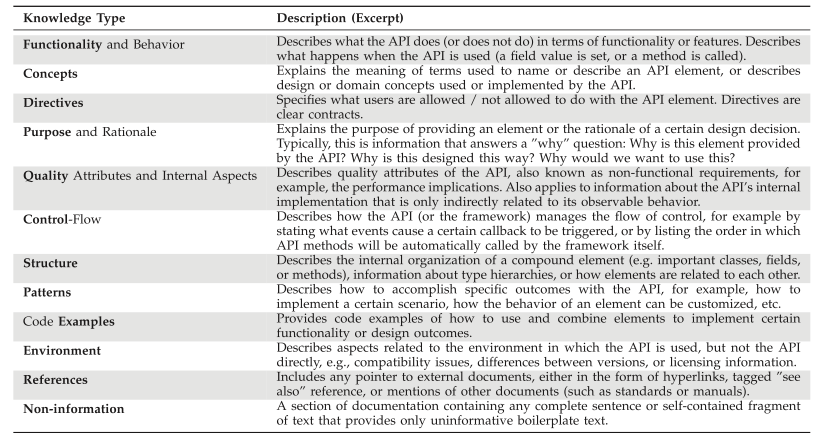
\includegraphics[width=1.1\textwidth]{pictures/knowledgetypes_original.png}
\caption[Wissenstypen in \cite{MaalejRobillard}]{Wissenstypen in \cite{MaalejRobillard}}
\label{fig:Wissenstypen_original}
\end{figure}
Die Vorgehensweise sah vor, dass die Gutachter f�r jeden Wissenstyp bestimmen, ob dieser in der vorgelegten Einheit vorkommt oder nicht. Hierzu konnten f�r jede Einheit die verschiedenen Wissenstypen mit Hilfe von "`CheckBoxes"' angekreuzt werden. 
Jede Einheit wurde von 2 Gutachtern unabh�ngig bewertet. Die Einheiten wurden in drei verschiedene Kategorieren aufgeteilt: 
\begin{enumerate}
\item Module [engl. modules] (entsprechen "`packages"' in Java und "`assemblies"' in .NET)
\item Typen [engl. types] (vor allem Klassen und Schnittstellen)
\item Mitglieder [engl. members] (Felder und Methoden)
\end{enumerate}
Die Einheiten der Kategorie "`Module"' wurden auf Grund der geringen Anzahl, der Unterschiedlichkeit (vor allem bzgl. der L�nge) in Java und .NET und des geringen Informatinosgehalts bei .NET dann aber nicht analysiert. Damit beschr�nkt sich die Original-Studie also auf Typen und Mitglieder. Die Stichprobe �ber die verbleibenden vier Kategorien (zwei je Programmiersprache) wurden mit 95\% Konfidenzintervall und 2,5\% Fehlerspanne gezogen, so dass insgesammt 5.575 Einheiten (431.136 W�rter) zuf�llig ausgew�hlt und auf 17 Gutachter verteilt wurden. \\
So sind insgesamt $5.574 * 2 = 11,148  $ Bewertungen vorgenommen worden. Diese wurden dann im Hinblick auf die �bereinstimmung unter den Gutachtern und bez�glich der Wissenstypen analysiert. Ebenso wurden Auswertungen �ber die F�lle getroffen, in denen sich zwei Gutachter uneinig waren. Zudem konnten so Aussagen dar�ber getroffen werden, welche Wissenstypen bei welcher Einheitskategorie wie h�ufig vorkommen und ob bestimmte Wissenstypen mit einander korrelieren, also  ob z.B. der Typ "'Structure"' h�ufig zusammen mit "`Functionality and Behaviour"' auftritt. Ebenso wurde analysiert, ob und wie ein Zusammenhang zwischen der Anzahl der gefundenen Wissenstypen und der L�nge der Einheiten besteht. \\
Besonders die vorgestellten Wissenstypen und das Kodier-Handbuch [Coding Guide] waren f�r diese Folgestudie sehr n�tzlich und wurden deswegen �bernommen und angepasst. 

\subsection{Kodier-Handbuch}
Das in der Original-Studie \cite{MaalejRobillard} verwendete Kodier-Handbuch findet auch in dieser Studie Verwendung, um von allen Gutachtern die selben bzw. sehr �hnliche Ergebnisse erwarten zu k�nnen. Es dient als Anleitung bei der Bewertung der Einheiten. W�hrend der Gro�teil des Handbuchs �bernommen wurde und unver�ndert bliebt, gab es jedoch ein paar wesentliche Anpassungen. 

\subsubsection{Markierungen}
\label{sec:Markierungen}
Der wichtigste Unterschied zu dem originalen Kodier-Handbuch \cite{codingguide_orig} ist, dass die Gutachtern nicht nur pro Einheit bewerten sollen, ob bestimmte Wissenstypen vorhanden sind, sondern Markierungen in einer Einheit vornehmen und pro Markierung einen Typ festlegen. Wie mit einem Textmarker soll jede Einheit vollst�ndig bearbeitet werden und abschlie�end jedes Zeichen (mit wenigen Ausnahmen) markiert sein. Dies f�hrt zu erg�nzenten Regeln �ber :
\begin{itemize}
\item Die Art Markierungen vorzunehmen
\item Der L�nge von Markierungen
\item Die Notwendigkeit von Doppelmarkierungen in einem Segment
\end{itemize}
Diese �nderungen wurden im ersten Absatz des Kodier-Handbuchs \cite{codingguide_new} wie folgt formuliert: 
\begin{shaded}
You will be presented with documentation blocks extracted from API reference documentation (Javadocs and the like). For each block, you will be also presented with the name of its corresponding package/namespace, class, method, or field. Your task is to read each block carefully and evaluate where the block contains knowledge of the different types described below. Apply the following rules when doing so:
\begin{itemize}
\item Consider the documentation initially one paragraph at a time. If the paragraph contains only information of one knowledge type, mark the whole paragraph with that type in one stretch.
Never mark more than one paragraph at once.
\item If multiple knowledge types mix within the paragraph, mark a contiguous stretch of one or more sentences with one type and the next stretch with another.
\item If necessary, treat subsentences connected with conjunctions such as "`and"', "`or"', "`but"', or with colon or semicolon like complete sentences.
\item A sentence (or such subsentence) as a whole is never marked with more than one type, but sometimes phrases within the sentence will require a separate marking with a different type. Double-marking the same text with two types is allowed (and required) in this case. To create such annotations uniformly, we work in two passes:
\begin{itemize}
\item Pass 1: Prefer longer segments of a complete sentence or several. Annotate subsentences only rarely.
If a sentence contains knowledge of more than one type (which happens quite often), look if one of them is clearly dominant for the overall role of the sentence in the documentation block. If so, annotate only that dominant type to the whole sentence and do not annotate any of the other types yet.
\item Pass 2: After pass 1, many relevant annotations will be missing. We now add those on top of the pass 1 annotations as double annotations. For the double annotations, we still prefer complete subsentences where possible (or other clearly delineated parts such as parentheses), but choose the shorter of two possibilities whenever we are unsure.
\end{itemize}
\item Rate the knowledge type as true only if there is clear evidence that knowledge of that type is present in the stretch.
If you have doubts, consult the type's definition below.
If the doubts do not disappear, do not annotate that type.
\item However, all text of the documentation must be marked with a type. (Only handwritten documentation, not the signature itself and not the placeholders [Something removed here] that indicate left-out nested documentation blocks).
\end{itemize}
Read (and re-read whenever needed) the following descriptions very carefully. They explain how to recognize each knowledge type.
\end{shaded}

\subsubsection{Kleinere �nderungen}
Zudem waren einige kleine �nderungen notwendig, die sich entweder aus dem Stil der Python-Dokumentation ergeben oder als sinnvoller bei der Bewertung von Einheiten ergeben haben. Folgende Semantische �nderungen gab es dabei: 

\begin{itemize}
\item Informationen �ber bestimmten Input einer Funktion oder Methode, welcher zu einer "`Exception"' f�hrt (und nur dann), soll als "`Directive"' und nicht als "`Functionality and Behavior"' markiert werden. 
\item Die simple Nennung von g�ltigen Parametertypen wird als nicht als "`Directive"' angesehen, sofern nicht  Schl�sselw�rter wie "`must"' oder "`have to"' etc. verwendet werden.
\item Der Ausdruck "`Changed in version x.y."' soll als "`Environment"' markiert werden. Der darauf anschlie�end Text kann ebenfalls "`Environment"' sein, muss es aber nicht. 
\item Platzhalter der Form "`[Something removed here]"' sollen nicht markiert und bewertet werden, da diese lediglich auf ausgelassene, verschachtelte Einheiten hinweisen (siehe Abschnitt "`Extrahierer"')
\item Der Wissenstyp "`Structure"' wird treffender in "`Structure and Relationship"' umbenannt. 
\end{itemize}



      
\section{Konzeption}
In diesem Abschnitt werden grundlegende Faktoren und Vorgehenweisen erl�utert, die w�hrend der Bachelorarbeit wichtig geworden sind. 
Diese betreffen sowohl die Beschaffenheit der Dokumentionseinheiten als auch die Stichprobenziehung und der daraus resultierende Zeitaufwand f�r die Gutachter. 
\subsection{Dokumentationseinheiten}
Mit Dokumentationseinheiten werden die Teilabschnitte aus der Dokumentation bezeichnet, die ein Gutachter f�r die Bewertung zusammenh�ngend angezeigt bekommt. 
Diese Einheiten wurden anhand der HTML-Syntax in der Original-Dokumentation bestimmt. Es sind folgende Kategorien mit den dazugeh�rigen HTML?Syntaxen aufgetreten:
\begin{enumerate}
\item Methoden (engl. methods)
\begin{itemize}
\item <dl class=\grqq method\grqq>  Methodeninhalt </dl>
\item <dl class=\grqq classmethod\grqq>  Methodeninhalt </dl>
\item <dl class=\grqq staticmethod\grqq>  Methodeninhalt </dl>
\item <dl class=\grqq function\grqq>  Methodeninhalt </dl>

\end{itemize}
\item Felder (engl. fields)
\begin{itemize}
\item <dl class=\grqq attribute\grqq>  Feldinhalt </dl>
\item <dl class=\grqq data\grqq>  Feldinhalt </dl>
\end{itemize}
\item Module (engl. modules)
\begin{itemize}
\item <div class=\grqq section\grqq>  Modulinhalt </div>
\end{itemize}
\item Klassen (engl. classes)
\begin{itemize}
\item <dl class=\grqq class\grqq>  Klasseninhalt </dl>
\item <dl class=\grqq exception\grqq>  Klasseninhalt </dl>
\end{itemize}
\item Beschreibungen (engl. describe)
\begin{itemize}
\item <dl class=\grqq describe\grqq> Beschreibungstext </dl>
\end{itemize}
\end{enumerate}

Die Kategorien unterscheiden sich von denen aus der Originalstudie in der Form, dass Felder und Methoden unabh�ngig von einander gef�hrt werden und zus�tzlich noch die Beschreibungselemente hinzugekommen sind. Anders als in der Originalstudie wird die Kategorie Module in der sp�teren Analyse nicht ausgelassen. 
Die Einheiten unterscheiden sich nebst Inhalt auch stark in ihrer Textl�nge. W�hrend die Einheiten der Kategorien 1, 2,  4  und 5 tendenziell eine kleine Textl�nge haben, sind die Module (3. Kategorie) in der Regel l�nger:
\begin{figure}[H]
\centering
 \begin{bchart}[step=500,max=3400,scale=1.4]
  \bcbar[text=Methoden]{1225}
  \bcbar[text=Felder]{619}
  \bcbar[text=Module]{3385}
  \bcbar[text=Klassen]{1233}
  \bcbar[value=Beschreibungen 482]{482}  
 \end{bchart}
 \caption[Durchschnittliche Textl�ngen je Kategorie]{Durchschnittliche Textl�ngen je Kategorie}
\end{figure}

Sehr gro�e Unterschiede gibt es zudem in der H�ufigkeit verschiedener Typen. Die wenigsten Vorkommen gibt es von den Einheiten "`describe"', "`classmethod"' und "`staticmethod"'. Einheiten des Types "`Method"' treten dagegen am allerh�ufigsten auf. Trotz des geringen Auftretens der "`describe"'-Elemente haben wir uns daf�r entschlossen, diese als eigene Kategorie zu behandeln, da diese bei den bisher behandelten Programmiersprachen (Java und .NET) nicht existent waren.
\begin{figure}[H]
\centering
 \begin{bchart}[step=300,max=2500,scale=1.4]
  \bcbar[value=staticmethod 2]{2}
  \bcbar[value=describe 17]{17}
  \bcbar[value=classmethod 26]{26}
  \bcbar[value=exception 240]{240}
  \bcbar[text=class]{614}
  \bcbar[text=attribute]{748}
  \bcbar[text=data]{762}
  \bcbar[text=section]{1595}
  \bcbar[text=function]{1802}  
  \bcbar[text=method]{2565}
 \end{bchart}
  \caption[Gesamth�ufigkeiten der Einheiten]{Gesamth�ufigkeiten der Einheiten}
\end{figure}

Die Verteilung auf der Kategorie-Ebene zeigt ebenfalls einen deutlichen �berschuss an Methoden: n�mlich fast drei?mal so viele wie es Felder gibt.  Auf Grund der einelementigen Kategorien "`Module"' und "`Beschreibungen"' decken sich hier deren H�ufigkeiten exakt mit denen der "`section"' und "`describe"'-Einheiten, so dass auch hier die Beschreibungselemente den geringsten Anteil darstellen. 
\begin{figure}[H]
 \begin{bchart}[step=1000,max=4400,scale=1.4]
  \bcbar[text=Methoden]{4395}
  \bcbar[text=Felder]{1510}
  \bcbar[text=Module]{1595}
  \bcbar[text=Klassen]{854}
  \bcbar[value=Beschreibungen 17]{17}  
 \end{bchart}
  \caption[Gesamth�ufigkeiten der Kategorien]{Gesamth�ufigkeiten der Kategorien}
\end{figure}

Mit Hilfe dieser Informationen k�nnen die im n�chsten Abschnitt beschriebenen Stichprobengr��en berechnet werden. 
\subsection{Stichprobe}
Um f�r alle Kategorien ein aussagekr�ftiges Ergebnis der sp�teren Begutachtungen erzielen zu k�nnen, werden die Stichproben unter Vorgabe von Konfidenzintervall und Fehlerspanne separat von einander pro Kategorie gezogen.  
Die minimale Anzahl der pro Kategorien zu ziehenden Einheiten wird mit dieser Formel berechnet \cite{Stichprobenziehung}:
\begin{displaymath}
MIN = \frac{n_0}{1+\frac{n_0-1}{Gesamtmenge}} 
\end{displaymath}
wobei $n_0$ wie folgt berechnet wird: 
\begin{displaymath}
n_0 = \frac{Z^{2}*0.25}{e^{2}}
\end{displaymath}
Dabei ist Z die Angabe des Konfidenzintervalls als z-score und e die tolerierte Fehlerrate. 
Bei einem Konfidenzintervall von 95 Prozent ist Z=1.96 \cite{Stichprobenziehung}. 
Mit einer Fehlerrate von 5 Prozent ergibt sich f�r $n_0 = 384,16$ und dadurch dann die folgenden minimale Stichprobengr��en f�r die jeweiligen Kategorien: \newline
\begin{figure}[H]
\centering
\begin{tabular}{|c||c|c|}\hline
   Kategorie & Gesamtmenge & Stichprobengr��e\\ \hline \hline
   Methoden & 4395 & 651 \\ \hline
   Felder & 1510 & 306\\ \hline
   Module & 1595 & 310 \\ \hline
   Klassen & 854 & 265 \\ \hline
   Beschreibungen & 17 & 16 \\ \hline \hline
   \textbf{Summe} & 8371 & 1548 \\ \hline
 \end{tabular}
\caption[Stichprobengr��en]{Stichprobengr��en}
\end{figure}
\subsection{Goldstichprobe}
Zudem wurde so eine weitere Stichprobe, die Goldstichprobe gezogen. Diese hat folgenden Zweck: 
\begin{itemize}
\item Absicherung der Messung bez�glich Korrektheit der Gutachterergebnisse und
\item Bestimmung eines Wertes f�r hohe Typisierungsqualit�t 
\end{itemize}
Diese Stichprobe wurde dann von vier unabh�ngigen Gutachtern der Freien Universit�t Berlin (Institut f�r Informatik) jeweils vollst�ndig typisiert. Diese Gutachter waren:
\begin{itemize}
\item Prof. Dr. Lutz Prechelt, AG Software Engineering
\item Holger Schmeisky, AG Software Engineering 
\item Franz Zieris, AG Software Engineering
\item Sven Wildermann, Verfasser dieser Bachelorarbeit
\end{itemize}
Wobei Holger Schmeisky und Franz Zieris zusammen eine Stichprobe bearbeitet haben. 
\newline
Die Gr��e dieser Stichprobe wurde auf 2 Prozent der Gesamtmenge aller Einheiten festgelegt, damit bei Beibehaltung einer repr�sentativen Gr��e der Aufwand im Rahmen blieb. F�r die einzelnen Kategorien ergaben sich somit folgende Mengen: 
\begin{figure}[H]
\centering
\begin{tabular}{|c||c|c|}\hline
   Kategorie & Gesamtmenge & Stichprobengr��e\\ \hline \hline
   Methoden & 4395 & 88 \\ \hline
   Felder & 1510 & 30 \\ \hline
   Module & 1595 & 32 \\ \hline
   Klassen & 854 & 17 \\ \hline
   Beschreibungen & 17 & 1 \\ \hline \hline
   \textbf{Summe} & 8371 & 168 \\ \hline
 \end{tabular}
\caption[Goldstichprobengr��en]{Goldstichprobengr��en}
\end{figure}
Dabei wurde der Wert f�r die Kategorie "`Beschreibungen"' um eins erh�ht, da diese Elemente sonst �berhaupt nicht in der Goldstichprobe vorgekommen w�ren. 
\subsection{Zeitaufwand}
Da die Gutachter der Hauptstichprobe im Rahmen des Kurses "`Forschungspraktikum"' an der Freien Universit�t Berlin f�r f�nf ECTS \footnote{European Credit Transfer System} die Einheiten bewerten haben, sollte der Aufwand so verteilt werden, dass die ben�tigten Punkte erreicht werden, aber gleichzeitig der Zeitaufwand nicht �berschritten wird (ein ECTS entspricht etwa 25 bis 30 Arbeitsstunden). Hierf�r muss der Aufwand des Markierens pro Einheit gesch�tzt werden, so dass die Einheiten pro Gutachter festgelegt werden k�nnen. Diese �berlegungen sind auch schon in der Stichprobenziehung mit eingeflossen und haben dazu gef�hrt, dass die Fehlerrate auf 5 Prozent gesetzt wurde. Da vor dem Start noch eine intensive Einarbeitung inklusive Hausarbeiten durchgef�hrt wurde, sind f�r die eigentliche Bewertung der Einheiten noch drei ECTS pro Student veranschlagt worden. Dadurch, dass jede Einheit von zwei Gutachtern bewertet werden sollte, mussten vorher die Stichprobengr��en mit zwei multipliziert werden, um die Gesamtanzahl der Bewertungen zu erhalten. Diese wurde dann auf die sieben Studenten verteilt (in der Tabelle wurde gerundet) und mit einem grob gesch�tzten, durchschnittlichen Zeitaufwand pro Einheit multipliziert: 
\begin{figure}[H]
\centering
\begin{tabular}{|c||c|c|c|c|}\hline
    & Anzahl der & Einheiten & Zeitaufwand & Zeitaufwand\\
   Kategorie & Bewertungen & pro Student & pro Einheit & gesamt\\ \hline \hline
   Methoden & 1302 & 186  & 5 min & 930 min \\ \hline
   Felder &  12 & 87 & 5 min & 435 min\\ \hline
   Module & 620 & 89 & 15 min & 1335 min\\ \hline
   Klassen &  530  & 76 & 10 min & 760 min\\ \hline
   Beschreibungen &  32 & 5 & 3 min & 15 min\\ \hline \hline
   \textbf{Summe} &  3096  & 443 & $\oslash 7.6$ min&  57,92 h\\ \hline
 \end{tabular}
\caption[Einheiten pro Student inkl. Zeitaufwand]{Einheiten pro Student}
\end{figure}
Zus�tzlich waren die Gutachter dazu angehalten, regelm��ig das KodierHandbuch zu lesen, um das �bergreifende Verst�ndnis nicht zu verlieren, sowie gelegentlich mit dem BugTracker\footnote{Ein System zur Erfassung von Defekten und Verbesserungsvorschl�gen} umzugehen. Hierf�r wurden zus�tzlich insgesamt noch etwa zehn bis zwanzig Arbeitsstunden invenstiert, wobei der tats�chliche Aufwand je Gutachter stark abweichen kann. \\
\newline
Analog kann auch der Zeitaufwand f�r die Bearbeitung der Goldstichprobe berechnet werden: 
\begin{figure}[H]
\centering
\begin{tabular}{|c||c|c|c|c|}\hline
                    & Anzahl der & Zeitaufwand & Zeitaufwand\\
   Kategorie & Einheiten &  pro Einheit & gesamt\\ \hline \hline
   Methoden & 88 &  5 min & 440 min \\ \hline
   Felder &  30 &  5 min & 150 min\\ \hline
   Module & 32 &  15 min & 480 min\\ \hline
   Klassen &  17  &  10 min & 170 min\\ \hline
   Beschreibungen &  1 & 3 min & 3 min\\ \hline \hline
   \textbf{Summe} &  168  & $\oslash 7.6$ min&  20,72 h \\ \hline
 \end{tabular}
\caption[Zeitaufwand f�r die Goldstichprobe]{Zeitaufwand f�r die Goldstichprobe}
\end{figure}
Da die Goldstichprobe drei mal bearbeitet wurde, ergibt sich so ein Gesamtaufwand f�r die Bearbeitung dieser von 62,16 Stunden.
Somit stellt sich die Frage, wie diese Einheiten aus der Original?Dokumentation verf�gbar gemacht werden.
\subsection{CADo-Tool vs. Eigenentwicklung}
Im Rahmen der Forschung von Maalej und Robillard \cite{MaalejRobillard} wurde ein Tool mit dem Namen CADo\footnote{Content Analysis for Software Documentation} geschaffen, welches folgende Werkzeuge und folgendee F�higkeiten mit sich bringt (�bersetzter Auszug) \cite{cado_tool} :
\begin{itemize}
\item API-Dokumentionen aus Online-Quellen extrahieren
\item Ziehen von zuf�lligen, stratifizierten Stichproben
\item Erstellung eines Codierungsschemas
\item Zuweisen von Einheiten zu Gutachtern
\item Berechnung der �bereinstimmung von Gutachtern
\end{itemize}
Aus der Perspektive des Gutachters birgt dieses Tool zus�tzlich noch folgende F�higkeiten \cite{cado_tool}:
\begin{itemize}
\item Online und offline login
\item Laden der zugewiesenen Einheiten
\item Einheiten typisieren (Codierungen hinzuf�gen)
\item Kodierhandbuch anzeigen 
\item Darstellung der Dokumentation
\item Kodiersitzungen zwischenspeichern und laden
\item Statistiken ansehen
\end{itemize}

Auf Grund der Vielzahl der f�r uns n�tzlichen F�higkeiten, stellte sich die Frage, ob dieses Werkzeug f�r diese Bachelorarbeit ebenfalls genutzt werden kann. 
Also habe ich dieses Werkzeug heruntergeladen und ausprobiert. Schon beim Herunterladen gab es Schwierigkeiten, da der auf der Website ver�ffentlichte Link ung�ltig war. Nach R�ckfragen bei den Autoren wurde dieser Misstand dann innerhalb weniger Tage von diesen behoben. \\
Der Test des Werkzeugs erwies sich dann ebenfalls als schwierig, da es noch in der alpha-Version\footnote{fr�hes Entwicklungsstadium ohne Garantie auf fehlerfreies funktionieren} und ohne Benutzerhandbuch vorlag. Zudem gab es bei m�glichen Fragen keinen einheitlichen Ansprechspartner und keine garantierte Antwortzeit der Entwickler, was ebenfalls zu einem h�herem Risikio in der Benutzung gef�hrt h�tte. \\
Somit haben wir es als sinnvoller angesehen, die f�r diese Bachelorabeit ben�tigten Werkzeuge selbst zu entwickeln. Dies hatte noch weitere Vorteile: 
\begin{itemize}
\item Grundverst�ndnis des vorliegenden Programmcodes
\item �nderungen des Grundkonzepts eher m�glich
\item schnellere Weiterentwicklung bei Bedarf
\item weniger Kommunikationsaufwand 
\end{itemize}
Wir haben uns entschlossen, diese Werkzeuge dann mittels Python zu entwicklen, um zus�tzlich noch Synergieeffekte bez�glich des Erlernens und Verstehens der Programmiersprache Python auszunutzen. 
\\ 
Da der Zugriff verteilt von den Rechnern der Gutachter erfolgen sollte, war die Entwicklung einer Website zu diesem Zweck sinnvoll, so dass Restriktionen bez�glich der Betriebssystemwahl ausger�umt werden konnten. \\
Diese Entscheidung f�hrte dazu, dass wir die Typisierungen �berhaupt anhand von Markierungen durchf�hren konnten (siehe Erl�uterung in Kapitel \ref{sec:Markierungen}), da wir so nicht mehr an den Gegebenheiten des CADo-Tools gebunden waren.

\section{Entwicklung und Durchf�hrung}
In diesem Kapitel wird zuerst erl�utert, wie das Extrahieren der Dokumentationseinheiten aus der Original?Pythondokumentation gemeistert wurde. Anschlie�end wird die Konzipierung und Umsetzung des Werkzeugs f�r die Markierung der Dokumentationseinheiten besprochen.
\subsection{Extrahierer}
Um die Dokumentationseinheiten aus der HTML-Dokumentation von Python zu erhalten, war es n�tig, einen Extrahierer als Skript zu schreiben. Dieser wurde in Python3 mit Hilfe von BeautifulSoup4 angefertigt. BeautifulSoup wurde genutzt, da es im Gegensatz zu regul�ren Ausdr�cken eine verst�ndlichere Syntax bietet, was zu einer leichteren und wartbareren Entwicklung f�hrt. \\
Entsprechend der Definitionen von Dokumentationseinheiten sollten also die HTML-Schnipsel getrennt von einander in eine Datenbank importiert werden. Diese Einheiten sind allerdings h�ufig geschachtelt, so dass eine Methodendeklaration in der Regel innerhalb einer Klassenbeschreibung vorkommt, welche wiederum innerhalb einer Sektion anzutreffen ist. Um Dopplungen bei der Typisierung zu vermeiden, wurden deswegen Platzhalter der Form "`[something removed here]"' an solchen Stellen eingebaut. Platzhalter haben einen wichtigen Vorteil gegen�ber dem einfachen Weggelassen dieser Elemente. So sieht auch der Gutachter, dass hier etwas von der Original-Dokumentation abweicht und kann sich somit die entstandenen L�cken erkl�ren. Dieser Fall tritt besonders h�ufig bei Sektionen auf, da diese in der Regel alle weiteren Elemente beinhalten. Aneinanderreihungen von Platzhaltern wurden wieder zu einem Platzhalter zusammengefasst.  \\
Eine m�gliche Struktur der Verschachtelung von Dokumentationseinheiten sieht ohne Beschr�nkung der Allgemeinheit so aus:  
\begin{figure}[H]
\centering
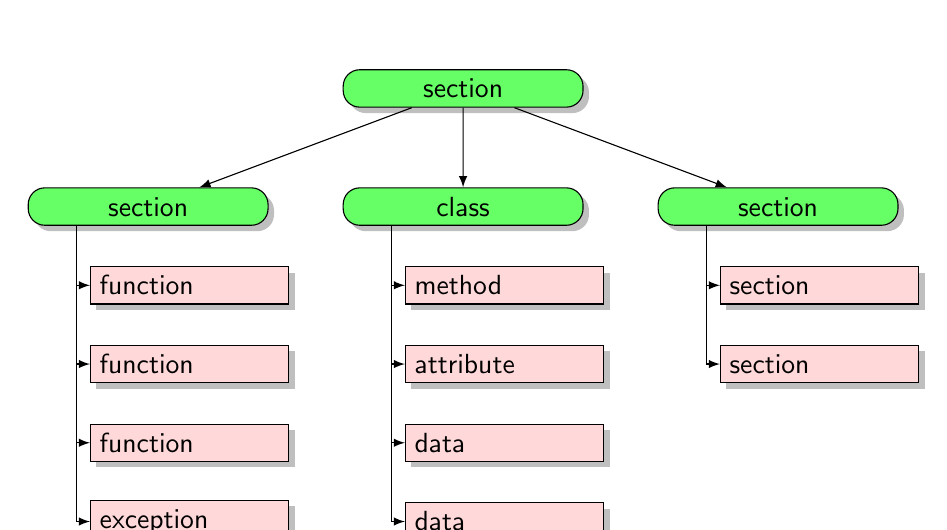
\begin{tikzpicture}[
  level 1/.style={sibling distance=40mm},
  edge from parent/.style={->,draw},
  >=latex]

% root of the the initial tree, level 1
\node[root] {section}
% The first level, as children of the initial tree
  child {node[level 2] (c1) {section}}
  child {node[level 2] (c2) {class}}
  child {node[level 2] (c3) {section}};

% The second level, relatively positioned nodes
\begin{scope}[every node/.style={level 3}]
\node [below of = c1, xshift=15pt] (c11) {function};
\node [below of = c11] (c12) {function};
\node [below of = c12] (c13) {function};
\node [below of = c13] (c14) {exception};

\node [below of = c2, xshift=15pt] (c21) {method};
\node [below of = c21] (c22) {attribute};
\node [below of = c22] (c23) {data};
\node [below of = c23] (c24) {data};

\node [below of = c3, xshift=15pt] (c31) {section};
\node [below of = c31] (c32) {section};
\end{scope}

% lines from each level 1 node to every one of its "children"
\foreach \value in {1,...,4}
  \draw[->] (c1.195) |- (c1\value.west);

\foreach \value in {1,...,4}
  \draw[->] (c2.195) |- (c2\value.west);

\foreach \value in {1,...,2}
  \draw[->] (c3.195) |- (c3\value.west);
\end{tikzpicture}
\caption{Beispielhafte Struktur der HTML-Elemente}
\label{fig:HTML-Elemente}
\end{figure}
\subsubsection{BeautifulSoup4}

F�r das Parsen der HTML-Einheiten wurde BeautifulSoup4 verwendet, da es ein hierf�r geschaffenes, m�chtiges Werkzeug darstellt und gleichzeitig auf Python basiert. Somit konnte ich Synergieeffekte nutzen und mich w�hrend des Schreibens am Skript weiter in Python einarbeiten. Zudem bietet der Einsatz von BeautifulSoup viele Vorteile gegen�ber dem Parsen mittels regul�ren Ausdr�cken. In erster Linie ist der Code lesbarer und verst�ndlicher, sowohl f�r den Entwickler selbst als auch f�r Dritte. Au�erdem gibt es eine ausf�hrliche Dokumentation inklusive zahlreicher Beispiele und auch die Community hinter BeautifulSoup ist gro� genug, um auf Internetportalen wie \href{http://www.stackoverflow.com}{Stackoverflow}\footnote{www.stackoverflow.com} Unterst�tzung erhalten zu k�nnen.  Die Implementierung selbst wird im nachfolgenden Kapitel erkl�rt. 

\subsubsection{Implementierung}

Bevor die n�tigen Schritte mit BeautifulSoup4 durchgef�hrt werden konnten, war es n�tig, die vollst�ndige Dokumentation herunterzuladen und die notwendigen Dateien ausfindig zu machen. Unter dem Link \url{https://docs.python.org/3.4/archives/python-3.4.1-docs-html.zip} ist die gesamte Dokumentation in einem HTML?Format verf�gbar. Interessant sind jedoch lediglich die Dateien in dem Unterordner "`library"' innerhalb dieser ZIP?Datei,  da Tutorials, Inhaltsverzeichnisse, FAQ und zus�tzliche Informationen analog der Studie von Maalej und Robillard \cite{MaalejRobillard} ausgeschlossen wurden. \newline

Der Extrahierer durchsucht anfangs alle Dateien in dem Unterordner "`library"' und f�gt den vollst�ndigen Pfad in eine Liste:
\lstinputlisting[language=Python, firstline=91, lastline=92]{code/extractor.py}

Aus jeder Datei wird dann ein BeautifulSoup-Objekt gemacht, welches die verschachtelte, innere HTML-Datenstruktur repr�sentiert:
\lstinputlisting[language=Python, firstline=94, lastline=95]{code/extractor.py}
Dieser Schritt ist n�tig, um im Anschluss mittels BeautifulSoup-API die einzelnen Dokumentationseinheiten extrahieren zu k�nnen. Hierf�r wird der Befehl find-all genutzt. Um eine einfache und fehlerfreie Bedienung zu erm�glichen, wurde eine Funktion geschrieben, die das DOM\footnote{Document Object Model}-Element samt Attribute entgegen nimmt:
\lstinputlisting[language=Python, firstline=84, lastline=86]{code/extractor.py}
Der Aufruf zum Parsen alle Elemente der Form 
\begin{lstlisting} 
<dl class="method"> 
Inhalt des Elements
</dl>
\end{lstlisting} 
und abspeichern dieser in einer Liste funktioniert dann wie folgt:
\lstinputlisting[language=Python, firstline=99, lastline=99]{code/extractor.py}
Dieser Schritt wurde analog f�r alle zehn verschiedenen Elementsytpen ausgef�hrt. 
Um sp�ter Aussagen �ber die Lage der Texte innerhalb einer Einheit zu erhalten, wurden zudem die Startoffsets der Elemente berechnet und sp�ter zusammen mit dem Endoffsets in der Datenbank abgelegt, wobei sich das Endoffset jeweils sehr leicht errechnen l�sst: 
$ Ende = Start + Laenge$.\\
F�r die Bestimmung der Startoffsets wurden die einzelnen Elemente in ihrer Datei mittels "`find"' aus BeautifulSoup gesucht und die R�ckgabe, also der Index an der Stelle des Auftretens, gespeichert. Auch hierf�r gibt es eine eigene Funktion, um den Aufruf lesbarer zu gestalten: \\ \\
\begin{minipage}{\textwidth}
 \lstinputlisting[language=Python, firstline=28, lastline=36]{code/extractor.py}
\end{minipage}
\newline
Au�erdem wurde dann f�r jedes Element das Vaterelement gesucht. Zum einen, um die Elemente sp�ter leichter wieder in die richtige Reihenfolge bringen zu k�nnen und zum anderen, um den Gutachtern die M�glichkeit zu geben, sich den engeren Kontext, in dem die zu bewertende Einheit steht, genauer anzusehen: 
 \lstinputlisting[language=Python, firstline=63, lastline=65]{code/extractor.py}
Wegen der bereits erw�hnten, verschachelten HTML-Struktur der Elemente musste ein Weg gefunden werden, um zu verhindern, dass ein inneres Element zweimal von den Gutachtern typisiert wird. Also wurden alle Vorkommen von inneren Elementen in den �u�eren Elemente durch folgende Platzhalter ersetzt: 
  \lstinputlisting[language=Python, firstline=138, lastline=138]{code/extractor.py}
Da so in vielen F�llen, z.B. bei der Aufz�hlung von Methoden und Attributen,  seitenweise Platzhalter entstanden w�ren, wurden im Anschluss direkt aufeinander folgende Platzhalter wieder zu einem Platzhalter zusammengefasst:
  \lstinputlisting[language=Python, firstline=39, lastline=44]{code/extractor.py}
Die final zur Verf�gung stehenden Informationen wurden dann in einer Datenbank abgespeichert.

\subsection{Typisierungswebsite}
% Die Typisierungwebsite stellt den Zugang f�r alle Gutachtern zu den Dokumentationseinheiten dar.
\subsubsection{Anforderungen}
Damit die Einheiten von den Studenten typisiert werden konnten, musste ein Werkzeug geschaffen werden, welches folgende Eigenschaften aufweist. Die mit einem Stern markierten Eigenschaften sind optional:
\begin{itemize}
\item Ein- und Auslogfunktion
\item Betriebssystemunabh�ngige Online-Erreichbarkeit
\item Anzeige der dem Student zugewiesenen Einheiten
\item Markierung von Segementen und Zuweisung zu Informationstypen
\item Anzeige der gesetzten Markierungen * 
\item Anzeige der Anzahl noch verbleibender und schon gespeicherter Einheiten *
\item Anzeige der eigenen �bereinstimmung mit anderen Studenten * 
\end{itemize}

\subsubsection{Umsetzung}
F�r die Umsetzung der genannten Anforderungen wurde das Webframework "`Django"' verwendet ? da es auf "`Python"' basiert und es eine gro�e Community gibt, die im Zweifel bei Herausforderungen unterst�tzten k�nnen. F�r die Beantwortung der anf�nglichen Fragen haben wir das in Berlin stattfindende Meetup der Django User Group\footnote{http://www.meetup.com/django-user-group-berlin/} besucht. Dar�ber hinaus gibt es eine Vielzahl von M�glichkeiten, mit anderen Django-Entwicklern zu kommunizieren, wie �ber die Mailingliste\footnote{{https://groups.google.com/forum/\#!forum/django-de}} oder den IRC-Chat (deutsch/weltweit).
\paragraph{Navigationsleiste} $\;$ \\
Die Navigationsleiste soll dem jeweiligen Benutzer alle Funktionen und Seiten anzeigen, die er im Rahmen des Werkzeugs benutzen kann.
Links, die auf ein Ziel innerhalb des Werkezeugs f�hren, sind blau. Externe Links sind grau gestaltet. 
Administrator-Funktionalit�ten haben eine rote Linkfarbe und werden nur eingeloggten Administratoren angezeigt. Wenn ein Benutzer ohne Administrationsrechte dennoch auf einen Link ger�t, f�r dessen Inhalt er keine Berechtigung besitzt, wird eine entsprechende Benachrichtigung angezeigt.

\paragraph{Login} $\;$ \\
Der Login soll allen Gutachtern erm�glichen, sich mit einem individuellen Account anzumelden, um gesch�tzten Zugriff auf die Dokumentationseinheiten und die pers�nliche Statistik zu erhalten. Weiterhin sollen Administratoren sich �ber diese Maske anmelden k�nnen, um Zugriff auf Administratorfunktionalit�ten zu erhalten. \newline
Der Login-Bereich wurde mit Hilfe des bereits in Django vorhandenen Authentifizierungsmoduls gefertigt. Angepasst wurde das Design an das der restlichen Website. Da eine Funktion f�r das Zur�cksetzten des Passwortes nicht ben�tigt wurde, wurde diese auch nicht implementiert. 
\begin{figure}[H] 
\centering
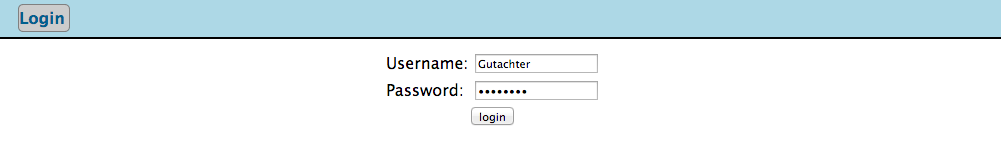
\includegraphics[width=1.0\textwidth]{pictures/login.png}
\caption[Login-Bereich]{Login-Bereich}
\label{fig:Login}
\end{figure}
$\;$ \\
\paragraph{Einheit typisieren} $\;$ \\
Nach dem Login wird der Gutachter direkt zu der n�chsten zu typisierenden Einheit weitergeleitet. 
Auf dieser werden neben der Navigation noch die Identifikationsnummer der Dokumentationseinheit, der Text der Einheit und Steuerungselemente angezeigt. Die Steuerungselemente sind im Einzelnen: 
\begin{enumerate}
\item Save ? speichert die aktuelle Markierung
\item Delete All ? l�scht alle gesetzten Markierungen des Gutachter bei dieser Einheit
\item Show Parent ? zeigt das direkte Vaterelement der Dokumentationseinheit an (siehe Abbildung \ref{fig:HTML-Elemente})
\item Show File ? zeigt die gesamte HTML-Datei, aus welcher diese Dokumentationseinheit stammt, im Original an
\end{enumerate}
Sobald der Text von dieser Einheit mit dem Mauscursor markiert wurde, erscheint ein Fenster f�r die Auswahl eines Wissenstypes. 
Die Position der Markierung wird dann zusammen mit dem Wissenstyp mit Hilfe von Javascript zwischengespeichert und dann beim Klicken auf "`save"' �ber Ajax als POST-request an den Controller\footnote{Entsprechend des "`Model View Controller"'-Musters} (in Django ist es die views.py) gesendet. Nach dem Speichern wird dann die n�chste Einheit angezeigt.  $\;$ \\
\begin{figure}[H] 
\centering
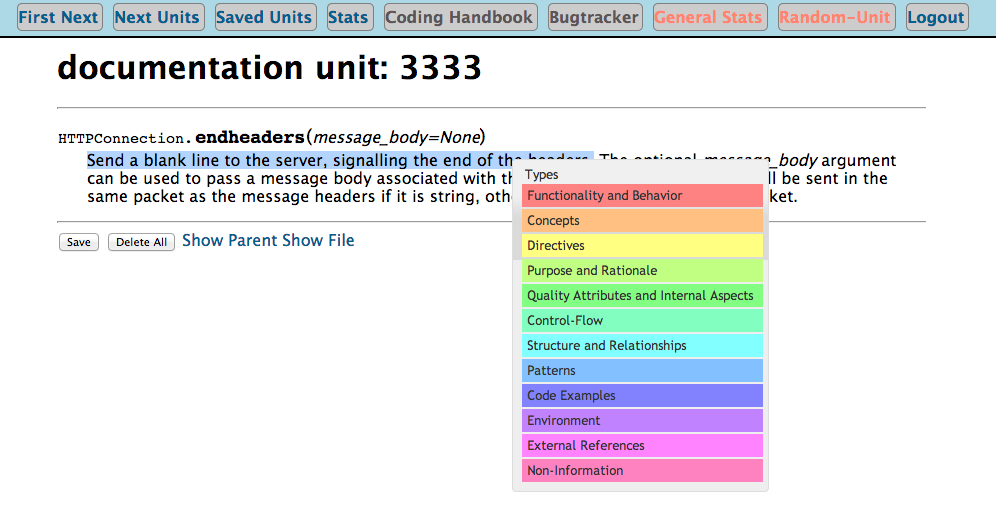
\includegraphics[width=1.0\textwidth]{pictures/marking.png}
\caption[Einheit typisieren]{Einheit typisieren}
\end{figure}
$\;$ \\
Die gesetzten Markierungen werden mit JavaScript farblich dargestellt. Bei Doppelmarkierungen wird die Farbe angezeigt, die zuletzt f�r die Auswahl gew�hlt wurde. Au�erdem erscheint unterhalb der Einheit eine Auflistung aller Markierungen. Sobald ein Element aus dieser Auflistung mit Mouse-Over\footnote{Bewegung des Maus-Cursor auf ein Element ohne es anzuklicken} ber�hrt wird, wird der damit verbundene, markierte Text rot und gestrichelt umrandet. Ein Klick auf dieses Element bewirkt das L�schen der angezeiten Markierung. 
\begin{figure}[H] 
\centering
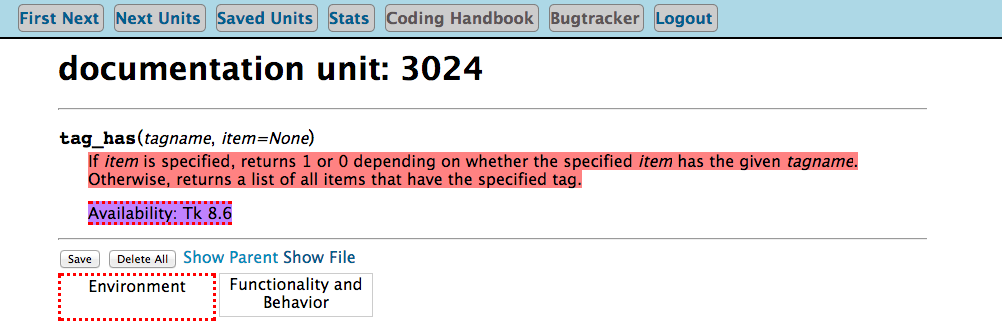
\includegraphics[width=1.0\textwidth]{pictures/single-delete.png}
\caption[Einheit typisieren (2)]{Einheit typisieren (2)}
\end{figure}
\paragraph{Noch nicht typisierte Einheiten} $\;$ \\
F�r den Fall, dass der Gutachter die zur Zeit n�chste Einheit noch nicht bewerten will, weil ihm diese f�r den Augenblick zu lang erscheint oder ihm gerade zu schwierig ist, kann er sich alle Einheiten auflisten, die noch typisiert werden m�ssen und davon eine ausw�hlen, die er als n�chstes bearbeiten m�chte. Dabei wird dem Gutachter die Identifikationsnummer, die Datei aus welcher die Einheit kommt und die Kategorie angezeigt. Der Klick auf eine Zeile f�hrt dann zu der Maske, in welcher die Einheit typisiert werden kann.
\begin{figure}[H] 
\centering
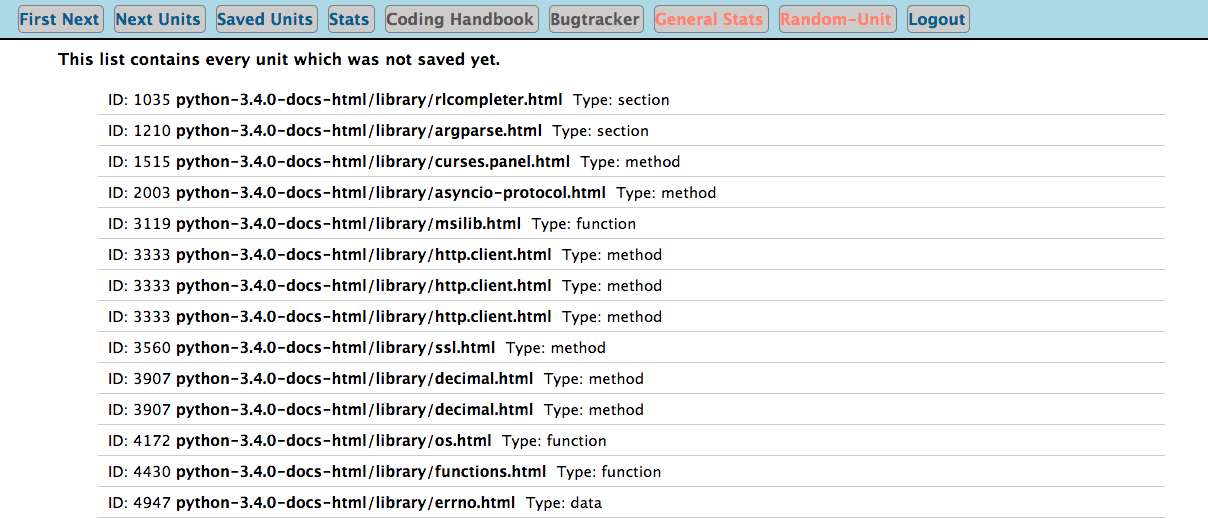
\includegraphics[width=1.0\textwidth]{pictures/list_of_next.png}
\caption[Noch nicht typisierte Einheiten]{Noch nicht typisierte Einheiten}
\end{figure}

\paragraph{Typisierte Einheiten} $\;$ \\
Zudem kann sich der Gutachter alle Einheiten auflisten lassen, die er bereits typisiert hat. Dabei werden alle Einheiten gelb hervorgehoben, die zu mehr als 25 Prozent und mehr als 100 Zeichen nicht markiert sind. Dies wurde so eingef�hrt, damit sehr kurze Einheiten, bei denen die nicht zu typisierende �berschrift fast genauso lang ist wie der eigentliche Text, nicht f�lschlich hervorgehoben werden. Bei den Textl�ngen wurden au�erdem die eingef�hrten Platzhalter herausgerechnet, da auch diese nicht markiert werden sollten.
So hat der Gutachter eine schnelle �bersicht �ber Einheiten, die er (in der Regel versehentlich) unvollst�ndig abgespeichert hat. 
Weiterhin wird f�r jede Einheit der Zeitstempel der vorhergegangenen Speicherung ausgegeben und bei Hervorhebung noch die Angabe in Prozent, wie viel des Textes nicht markiert ist. 
\begin{figure}[H] 
\centering
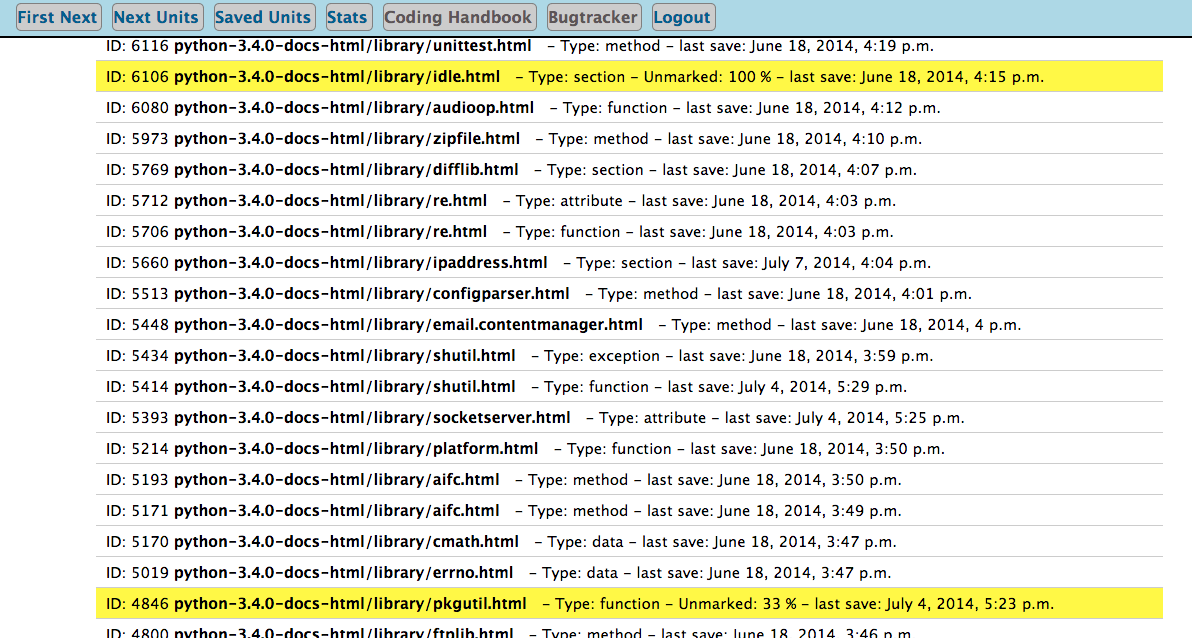
\includegraphics[width=1.0\textwidth]{pictures/einheiten-gespeichert.png}
\caption[Abgespeicherte Einheiten]{Abgespeicherte Einheiten}
\end{figure}
\paragraph{Pers�nliche Statistik} $\;$ \\
In der Statistik  (kurz: Stats) werdem dem angemeldeten Benutzer folgende Werte angezeigt: 
\begin{enumerate}
\item Anzahl insgesamt abgespeicherter Einheiten
\item Anzahl noch zu typisierender Einheiten (noch nicht abgespeichert)
\item Anzahl insgesamt zugewiesener Einheiten
\item Prozentuale �bereinstimmung der Markierungen mit den anderen Gutachtern (nur f�r die Gutachter der Hauptstichprobe)
\item Angabe der Anzahl der Einheiten, auf die sich die Berechnung der �bereinstimmung st�tzt
\end{enumerate}
Die 5. Angabe ist deswegen wichtig, da die Berechnung bei den schnellen Gutachtern sich auf weniger Einheiten st�tzt als schon markiert wurden. 
Das ist der Tatsache geschuldet, dass die Berechnung der �bereinstimmung pro Einheit erst erfolgen kann, wenn zwei Gutachter diese abgespeichert haben.\\
Diese Angaben werden einmal im Gesamten gemacht und dann anhand der letzten Speicherungsdaten f�r die letzten vierzehn, acht, vier und zwei Tage. Das hat den Vorteil, dass jeder Student schnell seinen eigenen Fortschritt f�r eine kurze Vergangenheit beobachten und dann auch ggf. erkennen kann, ob die �bereinstimmung mit anderen Gutachtern eher zu- oder abnimmt. \\ 
\begin{figure}[H] 
\centering
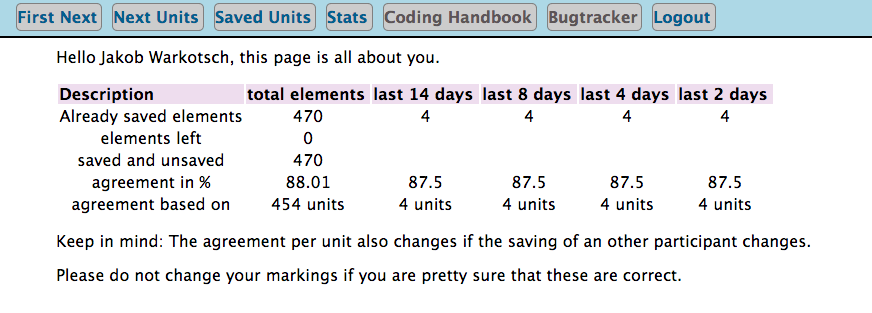
\includegraphics[width=1.0\textwidth]{pictures/personal_stats.png}
\caption[Pers�nliche Statistik]{Pers�nliche Statistik}
\end{figure}

\paragraph{Kodierhandbuch} $\;$ \\
Aus der Websitenavigation heraus kann direkt das Kodierhandbuch in einem neuen Tab ge�ffnet werden. Der Link verweist direkt auf die Website, die dieses enth�lt. 
Dieser direkte Link soll dazu f�hren, dass nochmaliges nachlesen m�glichst einfach gemacht wird und die Gutachter nicht erst noch nach dem Link suchen m�ssen. 
Der Link ist in der Navigation grau markiert, um zu verdeutlichen, dass es sich dabei um eine externe URL handelt.
\paragraph{Bugtracker} $\;$ \\
Ebenso kann der Bugtracker (gehosted bei bitbucket.org) schnell aus der Navigation heraus erreicht werden. Die Gutachter wurden angehalten, Schwierigkeiten in der Bedienung oder auftretende Fehler direkt dort zu melden, so dass alle Aufgaben bez�glich Verbesserung der Website zentral verwaltet werden k�nnen. Gegen�ber der �blichen E-Mail-Kommunikation hat dies den Vorteil, dass Gutachter erkennen k�nnen, wenn ein Fehler bereits gemeldet wurde, so dass Dubletten vermieden werden k�nnen. Au�erdem k�nnen Gutachter noch zus�tzliche Informationen zu den einzelnen Aufgaben liefern und f�r die Erledigung einer Aufgabe stimmen. \\
Weiterhin kann der interessierte Gutachter sich hier�ber den gesamten Quelltext der Website ansehen und so Ursache und L�sung der einzelnen Thematiken nachvollziehen, denn �nderungskommentare sind so in der Regel mit der l�senden �nderung im Quelltext verkn�pft. 
\begin{figure}[H] 
\centering
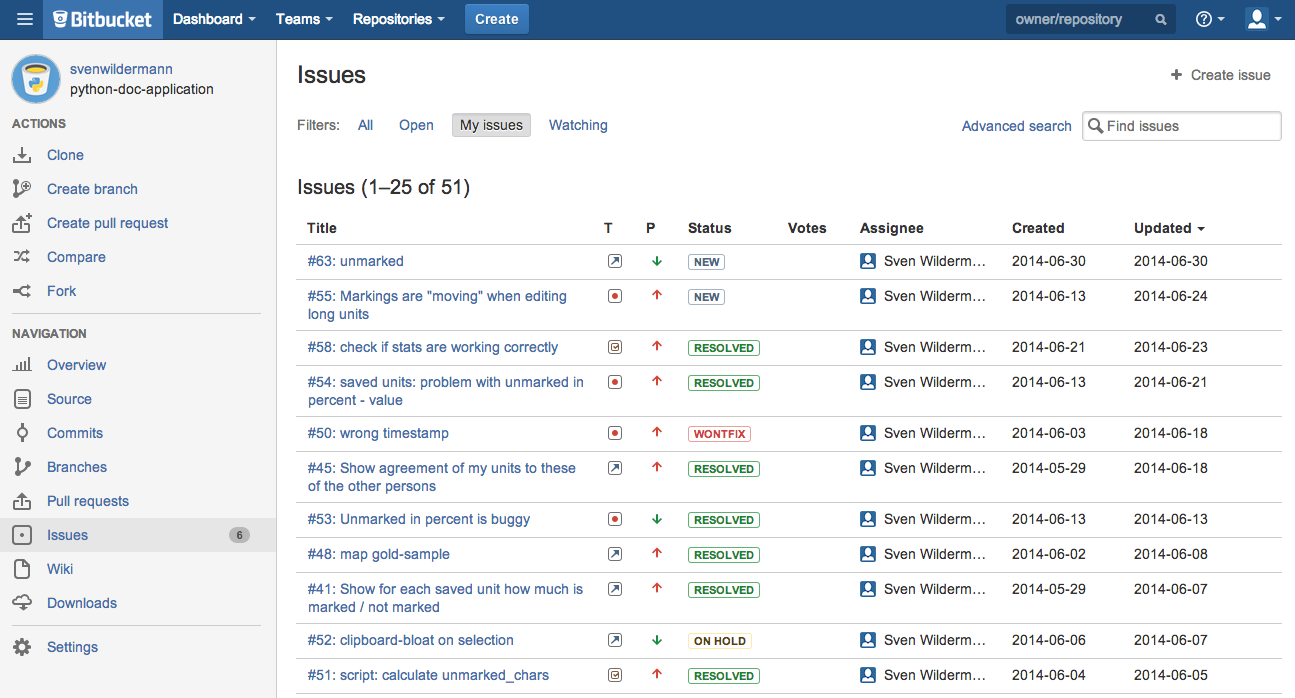
\includegraphics[width=1.0\textwidth]{pictures/bitbucket.png}
\caption[Bugtracker]{Bugtracker}
\end{figure}

\paragraph{Allgemeine Statistik} $\;$ \\
Die allgemeine Statistik ist eine reine Administratorfunktionalit�t und zeigt im wesentlichen die pers�nliche Statistik f�r alle Gutachter �bersichtlich an. Die �bereinstimmung unter den Gutachtern der Goldstichprobe wurde nicht berechnet und deswegen auch nicht angezeigt. Au�erdem weist diese Statistik noch die insgesamt zugewiesenen, gespeicherten (auch ohne Markierungen), markierten und nicht gespeicherten Einheiten an. Dabei werden Einheiten von Test- und Administratoraccounts mitberechnet. Da die einzelnen Gutachter hier mit Vornamen aufgelistet werden, wird auf die Einbindung eines Screenshots aus Datenschutzgr�nden verzichtet. 
\paragraph{Zuf�llige Einheit} $\;$ \\
Der "`Random Unit"'-Button ist ebenfalls eine reine Administratorfunktionalit�t und dient lediglich dem Testen. Grund f�r die Einf�hrung dieses Buttons war, dass bei Neuentwicklungen immer wieder anhand bisher unmarkierter Einheiten getestet werden und f�r die Zuweisung jedes Mal die Terminalumgebung genutzt werden musste. \\
Im Wesentlichen ist hinter dieser Funktion ein Bereich eingetragen, aus dem die Identifikationsnummern f�r die Dokumentationseinheiten stammen k�nnen. Aus diesem Bereich wird dann zuf�llig eine Nummer ausgew�hlt und als Einheit dem angemeldeten Benutzer zugewiesen. Dabei wurde keine R�cksicht darauf genommen, ob eine Einheit bereits markiert wurde oder nicht. Sollte eine Einheit erneut zugewiesen werden, die bereits dem Nutzer zugewiesen ist, taucht diese doppelt in den Listenansichten auf, wird aber trotzdem nur einmal bewertet. 
Da Markierungen von Administratoren sowieso nicht in der Auswertung ber�cksichtigt werden, ist dies unproblematisch. 
\paragraph{Logout} $\;$ \\
Die Logout-Funktionalit�t erm�glicht allen Gutachtern das sichere Abmelden von der Website. Umgesetzt wurde dieses analog zu der Login-Funktion mit dem in Django verf�gbaren Authentifizierungsmodul. Nach dem Logout wird der Benutzer wieder auf die Login-Seite umgeleitet. Im ausgeloggten Zustand kann nur der Login-Bereich besucht werden, alle anderen Funktionalit�ten (mit Ausnahme der externen Websites) sind nicht erreichbar. 

\paragraph{Hosting} $\;$ \\
Das gesamte Tool ist auf einem universit�ren Linux-Server des Instituts f�r Informatik gehostet. �ber die Eingabe einer URL im Browser war es somit von �berall aus erreichbar. Dabei kamen die Technologien Apache2, Django 1.6, GIT, Python3.2.3 und  PostegreSQL 9.3.5 zum Einsatz. Entwicklungen w�hrend der Bachelorarbeit wurden jederzeit lokal auf einem Notebook betrieben, dann erst mit Hilfe des Versionskontrollsystems GIT an das Repository geschickt und schlie�lich auf dem Server wieder heruntergeladen. Der Link zum Repository war die einzige ausgehende Verbindung au�erhalb des universit�ren Netzwerks, die akzeptiert wurde. Notwendige �nderungen an der Server-Datenbank wurden je nach Komplexit�t entweder manuell oder halb-automatisch mit Hilfe des Django-Werkzeugs "`South"' \footnote{South ist ein Werkzeug f�r Datenbankmigrationen innerhalb von Django-Applikationen.}durchgef�hrt.


\subsection{Gamification}
Um die Motivation der Gutachter zu erh�hen, wurden spielerische Elemente eingesetzt, auch "`Gamification"' genannt. 
Zum einen hatte jeder der Gutachter Zugriff auf seine pers�nliche Statistik und erhielt somit einen detailierten Fortschrittsbalken. Zum anderen wurden alle 14 Tage Auszeichnungen in Form von Gutscheinen f�r einen gro�en deutschen Versandhandel vergeben. Da die Typisierung aller Einheiten in etwa sechs Wochen gedauert hat, gab es drei Termine f�r Auszeichnungen.
Der 14-t�gige Rhythmus wurde allen Teilnehmern vorab bekannt geben. Bei jeder Auszeichnung wurden auch die nicht ausgezeichneten Teilnehmer �ber den Grund und die H�he der Belohnung anderer informiert. Dabei wurden unterschiedliche Fortschritte pr�miert: 
\begin{enumerate}
\item Nach den ersten zwei Wochen wurde lediglich der flei�igste Teilnehmer mit einen Gutschein belohnt, da die qualitative Auswertung noch nicht implementiert war.
\item Zwei Wochen sp�ter wurde sowohl der flei�igste Teilnehmer als auch der Teilnehmer mit der besten �bereinstimmung zu anderen Teilnehmern pr�miert.
\item Am Ende erhielten die beiden Teilnehmer mit den besten �bereinstimmungen jeweils einen Gutschein. Da alle vollst�ndig Einheiten typisiert wurden, ergab eine Pr�mierung des "`flei�igsten Teilnehmers"' keinen Sinn mehr.
\end{enumerate}
Insgesamt wurden Gutscheine im Wert von 30 Euro ausgezahlt. 

\subsection{Ungeplante �nderung}
\label{sec:Aenderung}
Nachdem etwa die H�lfte der Zeit f�r das Typisieren der Hauptstichprobe verstrichen war, wurde bekannt, dass einer der Gutachter (C1) aus privaten Gr�nden nur die H�lfte seiner Stichprobe bearbeiten wird. Daher mussten von den des Gutachtern zugewiesenen 442 Einheiten $221 = \frac{442}{2} $ auf alle anderen Gutachter verteilt werden. \\
Um den Mehraufwand f�r die Studenten m�glichst gering zu halten, haben wir uns dazu entschlossen, ebenfalls einen gleich gro�en Teil dieser Stichprobe zu typisieren. Zu den eigentlichen sieben Gutachtern wurden deswegen zwei weitere Gutachter-Accounts (sp�ter als C8 und C9 bezeichnet) hinzugef�gt, so dass insgesamt neun Gutachter an der Hauptstichprobe mitgewirkt haben. \\
Dabei wurde allerdings darauf geachtet, dass wir (C8/C9) keine Einheiten erhalten, die ebenfalls in der Goldstichprobe vorhanden sind, um zu vermeiden, dass unsere Markierungen mit den Ergebnissen aus der Goldstichprobe verglichen werden. Dies h�tte ansonsten zu einer Ergebnisverzerrung f�hren k�nnen. Im schlimmsten und unwahrscheinlichsten Fall w�ren so n�mlich 42 $(=2*21)$ von 168 Einheiten, also 25 Prozent, beim Vergleich mit der Goldstichprobe nicht mit den Ergebnissen von Studenten, sondern von den Kursleitern verglichen worden. \\
Jeder Gutachter (mit Ausnahme von C1) hat somit 27 bzw. 28 Einheiten $(\frac{221}{8}= 27.625) $ zus�tzlich bewertet. 

            

\section{Fazit /  Ergebnisse}
\subsection{Auswertung der Typisierungen}
\subsubsection{Konfusionen}
Bei der �berpr�fung der Vertr�glichkeit zweier Markierungen gibt es immer wieder den Fall, dass Gutachter A den Typ X, Gutachter B hingegen den Typ Y f�r sinnvoller h�lt. Daher wurde �berpr�ft, ob es Typen gibt, die besonders h�ufig mit einander verglichen werden. Mit Hilfe der folgenden SQL-Anweisung wurden alle aufgetretenen Konfusionen inklusive H�ufigkeit des Auftretens ausgegeben: 
\begin{lstlisting}[language=SQL] 
SELECT atype_id, btype_id, COUNT(*) 
FROM extractor_confusions 
GROUP BY atype_id, btype_id 
ORDER BY COUNT(*) DESC;
\end{lstlisting} 
Wenn jetzt noch die Reihenfolge ignoriert wird, also die Ergbenisse der Tupel (X,Y) mit denen von (Y,X) addiert werden, erh�lt man folgende Konfusionen, absteigend sortiert nach H�ufigkeiten des Auftretens. 
\begin{figure}[H]
\centering
\begin{tabular}{|c|c|c|c|}\hline
  Nr. & Typ A & Typ B & Anzahl \\ \hline \hline
  1 &Functionality and Behaviour      &    Structure and Relationships    &  439 \\ \hline
  2 &Functionality and Behaviour      &    Purpose and Rationale            &  271 \\ \hline
  3 & Functionality and Behaviour      &    Concepts                                &  243 \\ \hline
  4 &Functionality and Behaviour      &    Directives                               &  205 \\ \hline
  5 &Functionality and Behaviour      &    Non-Information                     &  177 \\ \hline
  6 & Functionality and Behaviour      &    Qual. Attributes, Intern. Aspects    &  176 \\ \hline
  7 & Functionality and Behaviour      &    Environment                           &  135 \\ \hline
  8 & Functionality and Behaviour      &    Patterns                                  &  107 \\ \hline
  9 &  Concepts                                  &    Structure and Relationships     &  105 \\ \hline
  10 & Purpose and Rationale               &    Structure and Relationships   &  90 \\ \hline
  11 & Patterns                                     &    Code Examples                      &  86 \\ \hline
  12 & Functionality and Behaviour       &    Control-Flow                          &  83 \\ \hline
  13 & Concepts     								&   Control-Flow 							& 79 \\ \hline
  14 &  Qual. Attributes, Intern. Aspects & Structure and Relationships & 70 \\ \hline
  15 & Purpose and Rationale 				& Patterns 									 & 67 \\ \hline
  16 & Structure and Relationships     & Patterns 										& 65 \\ \hline
  17 & Functionality and Behavior 			&  Code Examples 						& 63 \\ \hline
  18 &  Qual. Attributes, Intern. Aspects & Environment 					 & 60 \\ \hline
  19 & Concepts 									&  Qual. Attributes, Intern. Aspects & 59 \\ \hline
   20 & Directives 									& Structure and Relationships & 53 \\ \hline
   21 & Concepts 									& Patterns 								& 51 \\ \hline
 \end{tabular}
\caption[Konfusionsh�ufigkeiten]{Konfusionsh�ufigkeiten}
\end{figure} 
Aufgelistet werden die Konfusionen hier, sobald die untere Schranke von 50 Vorkommen erreicht wird. Um sich sp�ter leichter auf einzelne Konfusionen beziehen zu k�nnen, wurden diese durchnummeriert.
\subsection{Herausforderungen}
\section{Anhang}
\subsection{Technologien}
\subsubsection{Django}
\subsubsection{Python}
\subsubsection{BeautifulSoup4}
\subsubsection{Coffeescript}
\subsubsection{Postgres}
\subsubsection{Ajax}
\subsubsection{R}
\subsection{Kodierhandbuch - vollst�ndig}
\subsection{Glossar}
\begin{enumerate}
\item knowledge type / Informationstypen
\item API - in Implementierung des Extrahierer
\item DOM-Element

\end{enumerate}
      

\bibliographystyle{alpha}
\bibliography{bibliography}
\newpage



\end{document}
